\input sys/inputs.tex

\usepackage{tikz}

\begin{document}

\bigheading{Pohľadnice}

% \info{task_name}{infile}{outfile}{points}{timelimit}{memlimit}
% leave this values, if you are not interested
\info{posters}{stdin}{stdout}{100}{2000 ms}{1 GB}

Určite poznáte známu programátorskú súťaž IPSC, ktorú organizuje KSP. V rámci nej je možné získať
nejaký mínusový čas, ak nám pošlete peknú pohľadnicu. A za tie roky sa v KSP nahromadilo množstvo
pohľadníc zo všetkých kútov sveta, ktoré sme postupne vylepovali na našu stenu. Tá je už poriadne
zaprataná, dokonca sa niektoré pohľadnice navzájom musia prekrývať, aby sa tam vôbec zmestili.

A s novými pohľadnicami, ktoré prišli tento rok, nastáva problém, kam ich vylepiť. Maja, ktorá to má
na starosti navrhla nejaké možné pozície, Mišof je však skeptický, pretože si myslí, že prekryjú
príliš veľa zo starých pohľadníc. Pokúste sa teda zistiť pre každú pohľadnicu a jej pozíciu, akú
veľkú plochu starých pohľadníc prekryjú.

\heading{Úloha}

Na vstupe dostanete popis pozícii, na ktorých sú nalepené staré pohľadnice. Všetky pohľadnice sú
obĺžnikového tvaru a sú nalepené rovnobežne so súradnicovými osami. Následne dostanete popis
pohľadníc, ktoré chcete nalepiť aj s pozíciami, na ktoré budú nalepené. Zistite obsah plochy starých
pohľadníc, ktorý bude pokrytý novou pohľadnicou. Nové pohľadnice spracovávajte nezávisle od seba.

Keďže sa staré pohľadnice môžu prekrývať, ak nová pohľadnica zakryje ich prienik, rátajte túto časť
len raz.

\heading{Vstup}

Na prvom riadku vstupu je celé číslo $n$ ($1 \leq n \leq 100\,000$) -- počet starých pohľadníc.
Nasledujúcich $n$ riadkov, ktoré popisujú nalepené pohľadnice. Pohľadnica je popísaná štvoricou
čísiel $x_1$, $y_1$, $x_2$ a $y_2$ ($0 \leq x_1 < x_2 \leq 10^9$, $0 \leq y_1 < y_2 \leq 10^9$)
označujúce súradnice ľavého dolného a pravého horného rohu obdĺžnika.

Nasleduje číslo $m$ ($1 \leq m \leq 100\,000$) -- počet pohľadníc, ktoré chceme nalepiť. Nasleduje
$m$ riadkov, ktoré popisujú kam chceme nalepiť novú pohľadnicu. Popis je rovnaký ako predtým,
pomocou štyroch čísiel $x_1$, $y_1$, $x_2$ a $y_2$ ($0 \leq x_1 < x_2 \leq 10^9$, $0 \leq y_1 < y_2
\leq 10^9$).

V $12.5\%$ vstupoch bude platiť, že $n, m \leq 10$ a súradnice nebudú väčšie ako $100$.

V $25\%$ vstupoch bude platiť, že $n, m \leq 50$.

V $50\%$ vstupoch bude platiť, že $n, m \le 1000$.

V $50\%$ vstupoch nebudú súradnice väčšie ako $30\,000$.

\heading{Výstup}

Pre každú novú pohľadnicu vypíšte jedno celé číslo na samostatný riadok -- obsah plochy starých
pohľadníc, ktoré budú zakryté novou pohľadnicou.

\newpage

\heading{Príklad}


\sampleIN
2
0 1 3 5
2 3 6 6
2
1 0 5 4
4 2 7 7
\sampleCOMMENT
Na obrázku vidíte ako vyzerá stena v T2. Čiarkované obdĺžniky reprezentujú nové pohľadnice, vyplnené
obdĺžniku reprezentujú už nalepené pohľadnice.
\begin{center}
	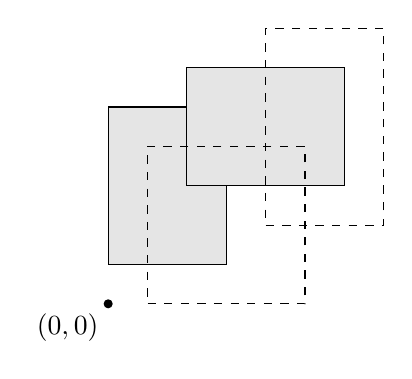
\begin{tikzpicture}[scale=0.5]
		\filldraw (0, 0) node[below left] {$(0, 0)$} circle(0.1);
		\filldraw[gray!20] (0, 1) -- (3, 1) -- (3, 5) -- (0, 5) -- cycle;
		\draw (0, 1) -- (3, 1) -- (3, 5) -- (0, 5) -- cycle;
		\filldraw[gray!20] (2, 3) -- (6, 3) -- (6, 6) -- (2, 6) -- cycle;
		\draw (2, 3) -- (6, 3) -- (6, 6) -- (2, 6) -- cycle;
		\draw[dashed] (1, 0) -- (5, 0) -- (5, 4) -- (1, 4) -- cycle;
		\draw[dashed] (4, 2) -- (7, 2) -- (7, 7) -- (4, 7) -- cycle;
	\end{tikzpicture}
\end{center}
\sampleOUT
8
6
\sampleCOMMENT
\sampleEND


\end{document}
